\begin{frame} \frametitle{\vspace*{0.5cm} Shock-driven fluid-fluid interfaces have been studied extensively}
  {\small
    \hfill%
    \begin{figure}
      \centering
      \begin{tikzpicture}%
        \node[anchor=south west,inner sep=0] (image) at (0,0) {
          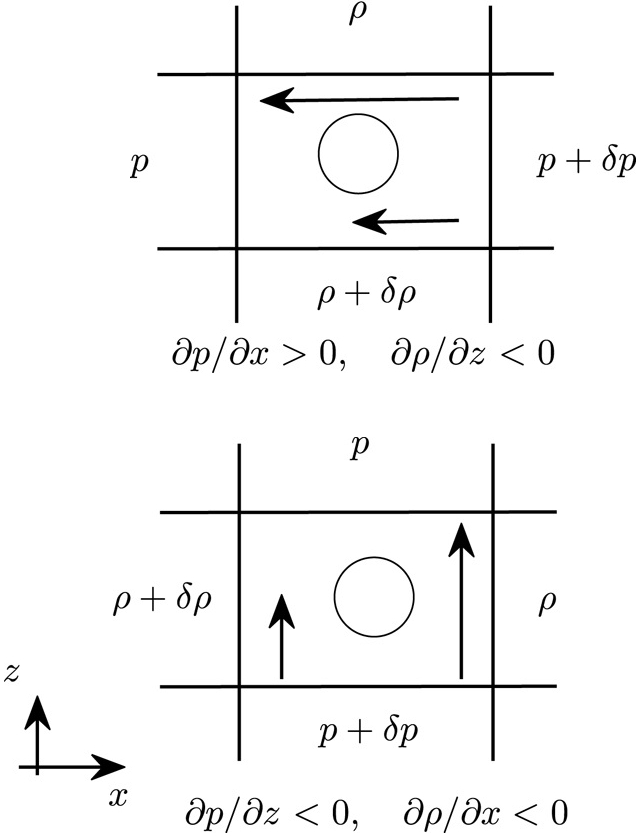
\includegraphics[height=0.5\textheight]{../figs/lung_figs/baroclinic_schematic_vertical}%
        };%
        \begin{scope}[x={(image.south east)},y={(image.north west)}]%
          \node[font=\tiny,right] at (0.05,-0.05) {\textcolor{black}{Adapted from \cite{Heifetz2015}}};%
        \end{scope}%  
      \end{tikzpicture}%
      \hfill%
      \begin{tikzpicture}%
        \node[anchor=south west,inner sep=0] (image) at (0,0) {
          \def\svgwidth{0.6\textwidth}%
          \import{../figs/lung_figs/}{brouillette_fig3_mod_compact.pdf_tex}\hfill%
        };%
        \begin{scope}[x={(image.south east)},y={(image.north west)}]%
          \node[font=\tiny,right] at (0.15,-0.05) {\textcolor{black}{Adapted from \cite{Brouillette2002}}};%
        \end{scope}%  
      \end{tikzpicture}%
    \end{figure}
    \hfill
    \begin{itemize}
    \item Shocks deposit baroclinic vorticity at perturbed fluid-fluid interfaces \citep{Drake2006}, which drives the interface perturbation to grow.
    \item This is the Richtymyer-Meshkov ``instability''.
    \item This problem is not well studied for acoustic waves.
    \end{itemize}
  }  
\end{frame}

%%% Local Variables:
%%% mode: latex
%%% TeX-master: "../main"
%%% End:
